\documentclass[a4paper,12pt]{scrreprt}
\usepackage[T1]{fontenc}
\usepackage[utf8]{inputenc}
\usepackage[ngerman]{babel}
\usepackage[table]{xcolor}% http://ctan.org/pkg/xcolor
\usepackage{tabu}
\usepackage{graphicx}



\begin{document}


\author{Dominik Backhausen \and Daniel Dimitrijevic \and Alexander Rieppel \and Thomas Traxler}
\subject{Pflichtenheft}
\title{LAN Yourself}
\date{\today}
\maketitle
\tableofcontents

\chapter{Projekt-Team}
	\begin{itemize}
	\item Dominik Backhausen (Teammitglied)
	\item Alexander Rieppel (Teammitglied)
	\item Daniel Dimitriejvic (Teammitglied)
	\item Thomas Traxler (Projektleiter)
	\end{itemize}
	
	
\chapter{Zielbestimmung}
	\begin{itemize}
	\item Peer-to-Peer Prinzip
	\item Erstellung von virtuellen LAN-Netzwerken
	\item intuitives GUI-Design
	\item Profilmanager für verschiedene Programme und zugehörige Programmprofile
	\item Einstellungsmenü für erweiterte Einstellungen
	\item Netzwerkteilnehmerliste
	\end{itemize}
	
	\section{Zulässige Erweiterungen}
	
	\begin{itemize}
	\item Weiterleitung der Internetverbindung eines Teilnehmers in sein LAN-Netzwerk
	\item Einstellung ob die Internetverbindung des LAN-Netzwerks oder die eigene verwendet werden soll
	\item Zugriffspunkt für die Internetverbindung in einem LAN-Netzwerk nach bestimmten Kriterien aussuchen lassen, wobei dies entweder manuell oder über einen Algorithmus erfordern kann
	\item Ports am Internetzugriffspunkt zu bestimmten Netzwerkteilnehmern weiterleiten
	\item Gemeinsame Ordner erstellen und bestimmten Netzwerkteilnehmern freigeben
	\item Onion-Routing (Pfadauswahl auch durch Kriterien möglich)
	\item Erweiterte Einstellungen für erfahrene Benutzer
	
	\end{itemize}
	
	\section{Unzulässige Erweiterungen / Nichtziele}
	
	\begin{itemize}
	\item Es ist kein Ziel die Software nach ihrer Fertigstellung proprietär zu vermarkten
	\item Es ist kein Ziel auf einer eigenen VPN-Lösung aufzusetzen
	
	\end{itemize}
	
	
\chapter{Produkteinsatz}
	
	\section{Anwendungsbereiche}
	 Die Software ist in erster Linie für Firmen gedacht die ein schnelles und einfaches VPN-Netzwerk benötigen. Dabei ist wichtig, dass verschiedenste Varianten dieses Szenarios denkbar sind, wie z.B. Mitarbeiter die international, auf allen Kontinenten verteilt, miteinander sicher kommunizieren müssen und gleichzeitig, im selben Netzwerk, Zugriff auf die internen Dienste der Firma benötigen (Server, Datenbank, etc.). Da die Software aber auch dafür ausgelegt ist, mit möglichst vielen verschiedenen Programmen zu funktionieren, sind die Anwendungsbereiche vielfältig. Deshalb ist sie nicht nur für Firmen, sondern auch für Privatpersonen interessant die ein VPN-Netzwerk einrichten wollen, aber dabei möglichst flexibel, benutzerfreundlich und sich die komplizierte Einrichtung eines VPN-Servers ersparen möchten. 
	 	
		
		
		
	\section{Zielgruppe}
	
	Generell kann man die Zielgruppe auf folgende großen Gruppen einschränken:
	\begin{itemize}
	\item Mitarbeiter die sich per VPN mit dem Intranet der Firma verbinden wollen um auf interne Server zuzugreifen und gleichzeitig möglichst sicher und international miteinander verbunden sein wollen.
	\item Private Personen mit dem Wunsch eines VPN-Netzwerks
	\end{itemize}
		
	\section{Betriebsbedingungen}
	Die einzige Anforderung die unser Produkt haben wird, ist ein PC mit einer funktionierenden Internetverbindung und einer installierten Version der verwendeten VPN-Software. Diese wird aber mit dem Programm mitgeliefert. Darüber hinaus wird unser Programm zunächst nur für Windows ausgelegt sein und daher keine Garantie für die Funktionalität auf anderen Systemen übernommen.
		
\chapter{Produktumgebung}
	
	\section{Software}
		
		Es ist bis auf die ausgewählte VPN-Basis keine andere Software von Nöten um unser Programm zu verwenden
		
	\section{Hardware}
		
	Die Software wird auf normalen PCs entwickelt und ist auch ausschließlich für jene gedacht. 
		
		
	\section{Produktschnittstellen}
		
	Fehlen??
	%Bitte hier ebenfalls noch die Funktionen anpassen und Funktionen die mit der Weiterleitung	der Internetverbindung zu tun haben in die Kann Ziele verschieben
		
\chapter{Produktfunktionen}
	Produktfunktionen einen Fehler bei der Ausführung. BITTE UNTERSUCHEN!!!
	
\chapter{Produktdaten}
	
	\textbf{/HD10/ Nickname}	
	
	Gespeicherter Nickname und Identität zur Authentifikation
	
	\textbf{/HD20/ Gespeicherte LAN-Netzwerke}
	
	LAN-Netzwerke die der Benutzer für die spätere Verwendung abgespeichert hat
	
	\textbf{/HD30/ Einstellungen}
	
	Vorgenommene Einstellungen in der Software
	
	\textbf{/HD40/ Programmprofile}
	
	Profile für Programmkompatibilität

\chapter{Produktleistungen}
\textbf{/LL10/ Optimierter Datenverkehr durch Peer-to-Peer}
	
	Da hier keine Server-Client Architektur verwendet wird, ist auch der Datenverkehr, der über einen einzigen Netzwerkteilnehmer geführt wird, deutlich geringer.
	
\textbf{/LL20/ Hohe Erweiterbarkeit der Software durch vorausschauend geplantes Programmdesign}
	
\textbf{/LL30/ Hohe Kompatibilität zu verschiedensten Programmen}
	
	Bei der Entwicklung der Software wird besonders darauf geachtet, dass sie mit verschiedensten Programmen kompatibel ist. Da dies natürlich nicht immer vom Programm selbst gewährleistet werden kann, wird es hierfür einen Profilmanager geben. Dieser ist speziell dafür gedacht Programmprofile zu Programmen zu erstellen die eine spezielle Konfiguration des Netzwerks oder des Netzwerkteilnehmers erfordern.
	
\textbf{/LL40/ Hohe Performanz}
	
	Hiermit ist sowohl Performanz innerhalb des Programms, als auch im Netzwerk gemeint.
	
	
	
	
\chapter{Benutzerschnittstelle}
	Bestehende Programme haben oft eine unzureichend intuitive oder nicht ausreichend erklärte Benutzeroberfläche in denen sich unerfahrene Benutzer oft nur sehr schwer zurechtfinden und einige Eingewöhnungszeit benötigen. Deshalb wird die Benutzerschnittstelle, aber auch das Programm selbst, besonders intuitiv und einfach verwendbar sein um die wichtigsten Funktionen möglichst einfach erreichen zu können. Die Software wird daher im Auslieferungszustand bereits ohne eine einzige Einstellung auskommen und kann bereits nach dem Start der Software verwendet werden.
	
	
	
\chapter{Qualitätsbestimmungen}
\begin{itemize}
	\item {\LARGE\textbf{Sicherheit}}\\
	Das Produkt wird hauptsächlich auf den Einsatz mit vielen Benutzer zugeschnitten. Um in dieser Gemeinschaft dem Abhören von übertragenen Daten vorzubeugen, wird besonders auf gute Sicherheitslösungen und Verschlüsselungsmechanismen viel Wert gelegt.
	\item {\LARGE\textbf{Benutzbarkeit}}\\
	Bei der Entwicklung wird äußerst viel Wert auf eine intuitive und einfache GUI gelegt, die aber sowohl was die Performanz, als auch das Design angeht schöne Ergebnisse liefert und damit in erster Linie dem Benutzer zugute kommt.
	\item {\LARGE\textbf{Effizienz}}\\
	Da bei unserem Programm auch mit vielen Benutzer gerechnet wird und diese auch viele Daten verschicken, muss unser Programm auch imstande sein diese Netzwerklast zu reduzieren und zu managen. Weiters ist es notwendig, dass die Software auch selbst schnell und effizient arbeitet. Daher wird bereits bei der Code- und GUI-Entwicklung auf möglichst geringe Ladezeiten geachtet und auf schnelle Befehlsdurchführung wertgelegt.
	\item {\LARGE\textbf{Erweiterbarkeit}}\\
	Wie bereits bei den Hauptleistungen erwähnt, ist vorgesehen das Programm so zu schreiben, dass zukünftige Erweiterungen der Software leicht möglich sind.
	\item {\LARGE\textbf{Übertragbarkeit}}	\\
	%Bitte zu überarbeiten da wie jetzt C++ statt Java benutzen
	\end{itemize}
\chapter{Globale Testfälle}
	
	\begin{figure}
\centering
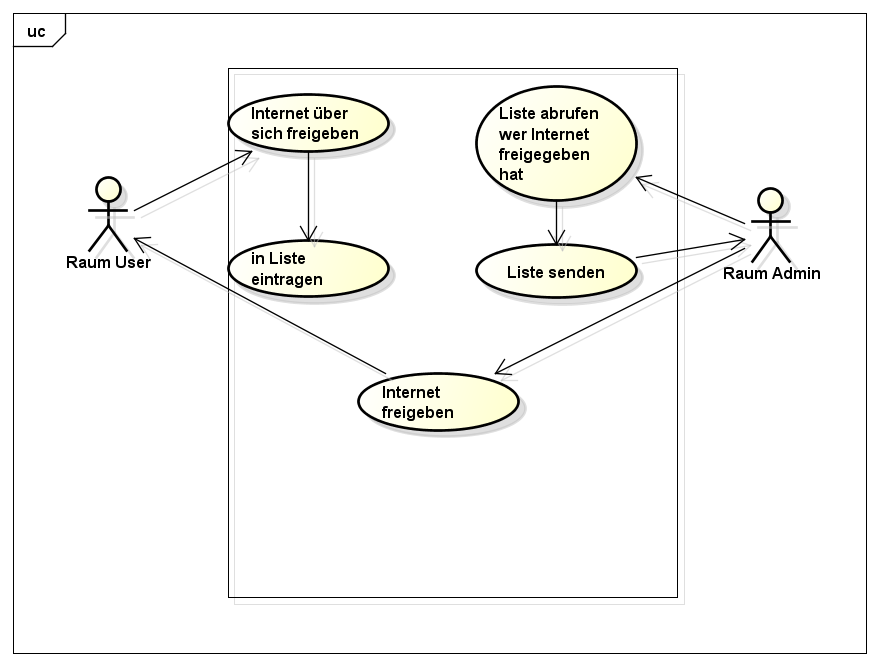
\includegraphics[width=0.7\linewidth]{C:/Users/Daniel/Desktop/Aufgaben/5ahitt/VPN_Internet_freigeben}
\caption{}
\label{fig:VPN_Internet_freigeben}
\end{figure}
\begin{figure}
\centering
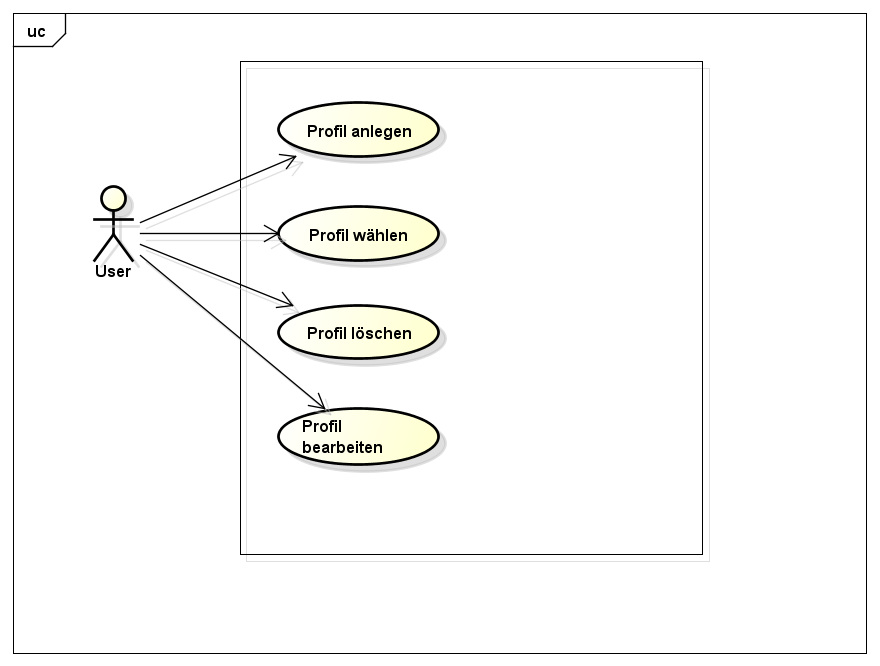
\includegraphics[width=0.7\linewidth]{C:/Users/Daniel/Desktop/Aufgaben/5ahitt/VPN_Profilemanager}
\caption{}
\label{fig:VPN_Profilemanager}
\end{figure}
\begin{figure}
\centering
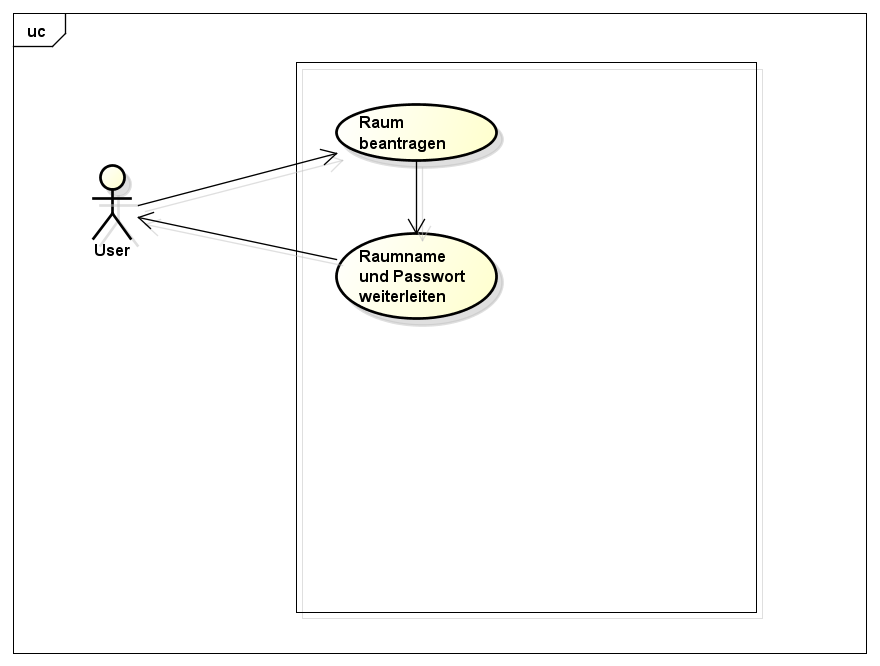
\includegraphics[width=0.7\linewidth]{C:/Users/Daniel/Desktop/Aufgaben/5ahitt/VPN_Raum_Beantragen}
\caption{}
\label{fig:VPN_Raum_Beantragen}
\end{figure}
\begin{figure}
\centering
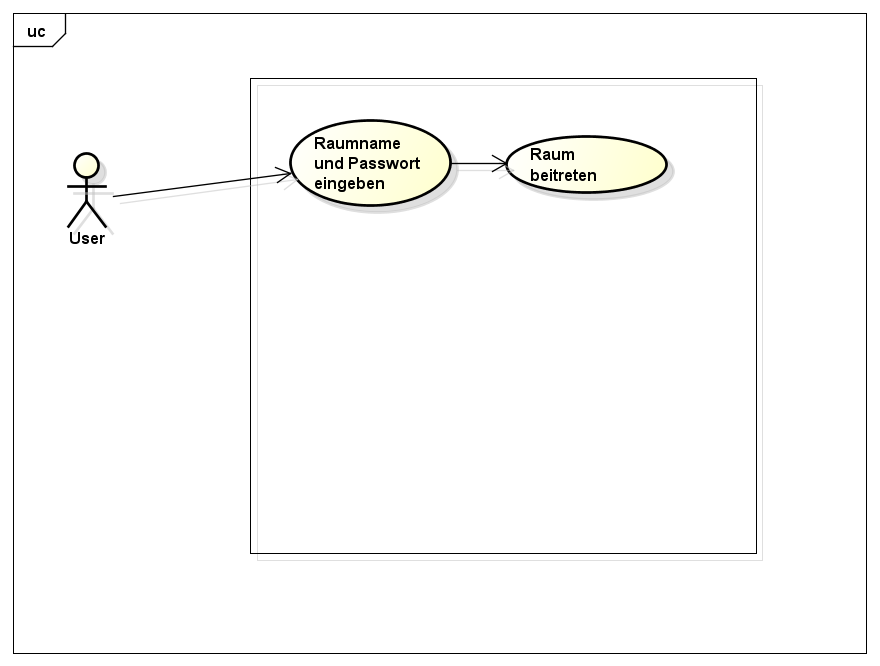
\includegraphics[width=0.7\linewidth]{C:/Users/Daniel/Desktop/Aufgaben/5ahitt/VPN_Raum_Beitreten}
\caption{}
\label{fig:VPN_Raum_Beitreten}
\end{figure}

	
\chapter{Entwicklungsumgebung}
	
	\section{Software}
		Zur Entwicklung der Software wird jeder seine Entwicklungsumgebung benutzen dürfen. Falls es zu Fehlern zwischen denn Entwicklungsumgebungen kommt werden wir uns auf eine einigen und nur mit dieser weiter arbeiten.\\		
		Visual Studio \\
		Code Blocks
		
		
		
	\section{Hardware}
		
		
		Die Software wird auf normalen PCs entwickelt und ist auch ausschließlich für jene gedacht.
		
		
		
\chapter{Projektplanung}



	
	
\end{document}